\item \points{2g}

In this question, our grader will evaluate the performance of your linear implementation on the test environment based on the code you have already developed in previous questions in this section (No additional code needs to be written for this question).

If you would like, you can observe the performance metrics of your model through running the following command:

\begin{lstlisting}
$ python run.py --config_filename=q2_linear
\end{lstlisting}

This should train your linear model on the test environment with the configuration defined in ~config/q2_linear.yml~. You may view the evaluation scores from your training run under the following directory ~results/q2_linear/~. We expect your implementation to achieve the optimal return on the test environment. Below we have provided a plot of scores which we expect the scores generated by your implementation to closely resemble:

\begin{figure}[H]
\centering
  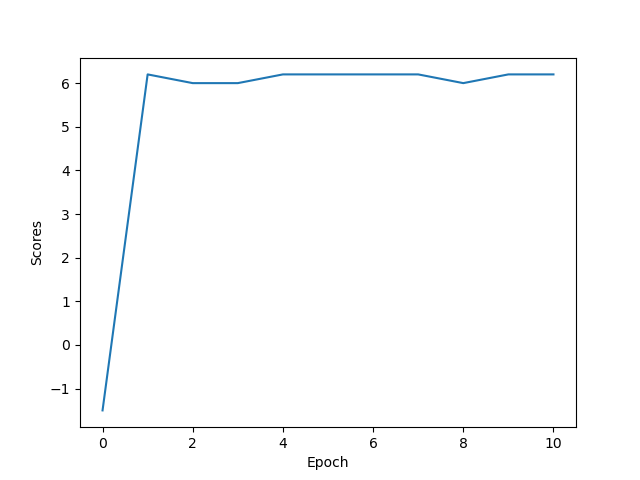
\includegraphics[width=.5\linewidth]{images/linear_test.png}
\end{figure}

\textit{Note: You will be need these results to provide responses to future questions which are made available online via Gradescope.}
\clearpage